\chapter{PQ-DTLS with Source Authentication and Data Integrity}

\section{Threat Model}
 – Adversary has access to quantum computer
 
 \section{Security Guarantee }
 – Integrity and Source authentication with PQ security
 
\section{DTLS with source auth and integrity }

Handshake uses PSK for mutual authentication(that creates secure session) and key exchange to create a master key for checking integrity of handshake finish messages.


Alternatively, handshake could have used key-exchange(DH or RSA) to create a master key for checking integrity and certificates for source auth.


Removal of data confidentiality, that is, data encryption and decryption.


This serves as DTLS with src auth and integrity only

\subsection{Security Claims }




\section{Integrating TESLA in DTLS with source auth and integrity (without PQ security)}

\subsection{Modified Handshake layer protocol – uses ECDSA signature }

As already presented, that TESLA can be integrated with DTLS by modification in handshake, removing confidentiality as shown in Figure \ref{hs}, with 181 Bytes overhead during handshake and 68 Bytes during application datagram record(considering RSA 1024 signature, HMAC-SHA-256 as PRF).The elements in \textcolor{red}{RED} are not included when the PSK key exchange algorithm is used(in authentication only mode) as described in \href{https://tools.ietf.org/html/rfc4279#section-2}{RFC 4279}. The dashed connection are part of TESLA message exchange.

Modifying handshake in DTLS is a bit tricky, as we want the data from TESLA to be protected and still be accepted by DTLS client and server. This is because DTLS client and server send a message flight "FINISHED", which contains MAC of previous message flights for integrity check. We need to make TESLA information be a part of this integrity check. \cite{tls-byte-explained}

 \begin{figure}[H]
    \centering
    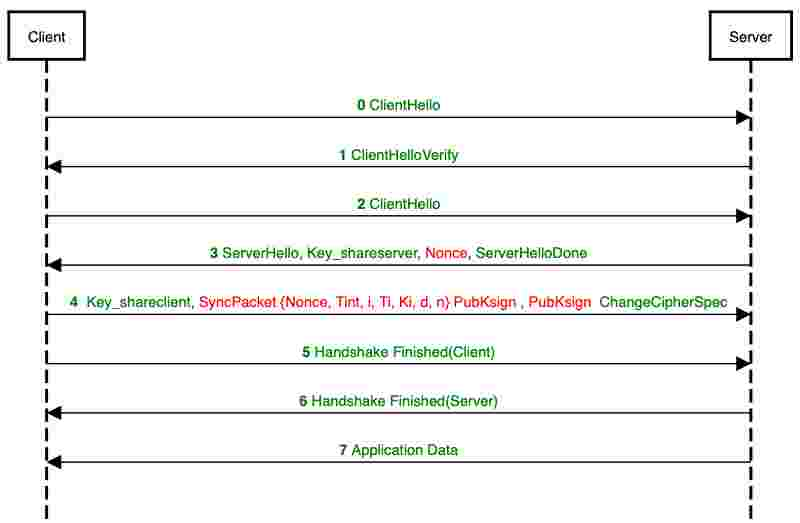
\includegraphics[height=10cm,width=16cm]{figures/hs.jpg}
    \caption{DTLS+TESLA Authentication mode using PSK}
    \label{hs}
\end{figure}
    

The two ways to modify the handshake are :
\begin{enumerate}
    \item Add message flights to existing handshake, maintaining the state of the peer(client/server).
    \item Adding the required messages to existing handshake flights, by modifying the maximum length of the header and/or message flight.
\end{enumerate}  


\textcolor{red}{We choose to work with changing the existing flights to accommodate TESLA packets. We add handshake maintaining state of the client and server after each message flight. Technically, there is no change in state of the original DTLS server or client, the handshake flights add TESLA data to the existing flights. }

We go ahead with the changing the existing handshake, this means that existing handshake message flights contains tesla messages.

\begin{enumerate}
    \item \textbf{ServerHello} contains \textbf{tesla synchronization request} with a nonce, a total of 32 Bytes addition to existing flight.
    
    \item \textbf{ClientKeyExchange} contains \textbf{tesla synchronization response} message with a nonce, a total of 181 Bytes addition to existing flight.
    
\end{enumerate}  

Figure \ref{hs-tesla-state} tracks state change in tinyDTLS, showing communication between the client and server.



\begin{figure}[H]
    \centering
    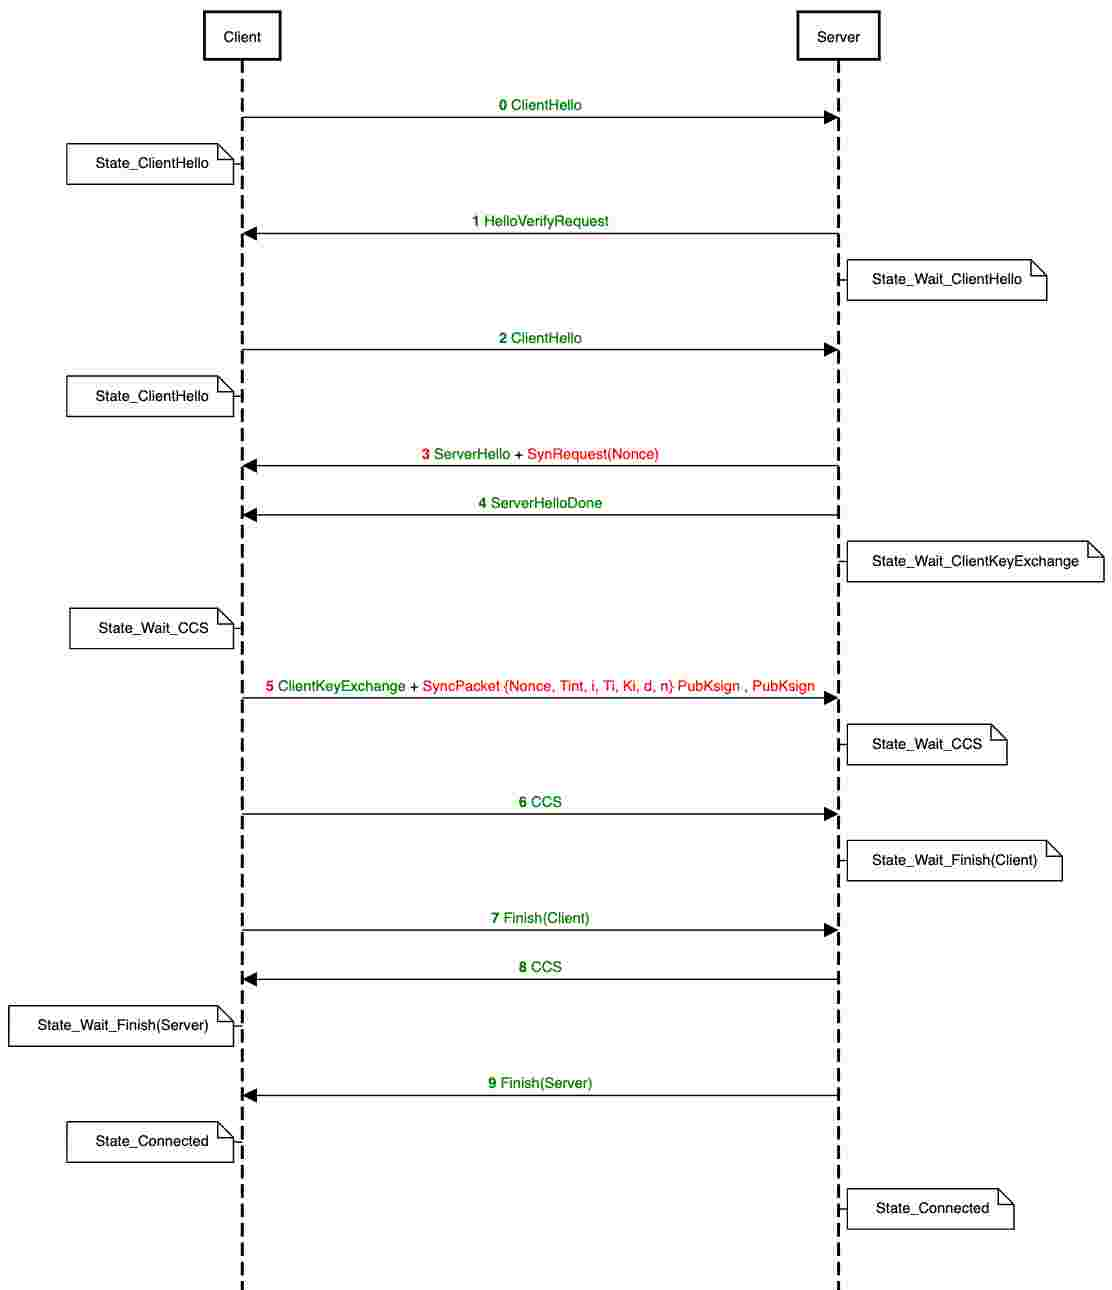
\includegraphics[height=20cm,width=16cm]{figures/hs-tesla-state.jpg}
    \caption{Stateful tinyDTLS with TESLA(Modify Existing Flights)}
    \label{hs-tesla-state}
    \end{figure}
    
    
    
\subsection{Modified record layer protocol}

\subsection{Security Claims}




\section{Integrating PQ-TESLA in DTLS with source auth and integrity}


\subsection{Modified Handshake layer protocol -uses K2SN-MSS}
\subsection{Modified record layer protocol}
\subsection{Security Claims}
Integrating PQ-TESLA in DTLS with source auth and integrity


\section{Security Analysis}